%\VignetteIndexEntry{RNA-Seq Report Template}
%\VignetteDepends{NBPSeq, baySeq, systemPipeR, ggplot2}
%\VignetteKeywords{DEGs, pipeline, reports}
%\VignettePackage{DEG.comparison}

% Latex compile
% Sweave("script_DEG.Rnw"); system("pdflatex script_DEG.tex; bibtex script_DEG; pdflatex script_DEG.tex; pdflatex script_DEG.tex")
% echo 'Sweave("script_DEG.Rnw")' | R --slave; echo 'Stangle("script_DEG.Rnw")' | R --slave; pdflatex script_DEG.tex;  bibtex script_DEG; pdflatex script_DEG.tex

\documentclass{article}
\RequirePackage{/home/cassol/R/x86_64-pc-linux-gnu-library/3.1/BiocStyle/resources/latex/Bioconductor}
\usepackage[authoryear,round]{natbib}
\bibliographystyle{plainnat}
\def\bibsection{\section{References}}

\usepackage{graphicx}
\usepackage{color}
\usepackage{hyperref}
\usepackage{url}
\usepackage{float}

%\newcommand{\comment}[1]{}
%\newcommand{\Rfunction}[1]{{\texttt{#1}}}
%\newcommand{\Robject}[1]{{\texttt{#1}}}
%\newcommand{\Rpackage}[1]{{\textit{#1}}}
%\newcommand{\Rmethod}[1]{{\texttt{#1}}}
\newcommand{\Rfunarg}[1]{{\texttt{#1}}}
%\newcommand{\Rclass}[1]{{\textit{#1}}}
	
% Define header and footer area with fandyhdr package (see: http://www.ctan.org/tex-archive/macros/latex/contrib/fancyhdr/fancyhdr.pdf)
\usepackage{fancyhdr}
\pagestyle{fancy}
\fancyhead{}
\fancyfoot{}
\rhead{\nouppercase{\leftmark}}
\lhead{\textit{systemPipeR RNA-Seq Report}}
\rfoot{\thepage}

%\parindent 0in

%\bibliographystyle{plainnat}

\usepackage{Sweave}
\begin{document}
\Sconcordance{concordance:script_DEG.tex:script_DEG.Rnw:%
1 9 1 1 4 27 1 1 5 4 1 1 0 21 1 1 2 4 0 1 2 1 1 1 2 4 0 1 2 2 1 1 2 1 0 2 1 24 0 1 2 %
9 1 1 2 1 0 4 1 3 0 1 2 9 1 1 2 1 0 1 1 3 0 2 2 1 0 2 1 1 2 4 0 2 2 4 0 1 2 2 1 1 2 %
1 0 1 1 3 0 1 3 11 0 1 2 2 1 1 4 6 0 1 2 3 1 1 2 1 0 4 1 1 4 3 0 5 1 3 0 2 2 4 0 2 2 %
4 0 1 2 2 1 1 2 1 0 7 1 3 0 1 2 8 1 1 2 1 0 4 1 3 0 1 2 1 1 1 2 1 0 4 1 3 0 1 2 1 1 %
1 2 1 0 4 1 3 0 1 2 7 1 1 2 1 0 4 1 3 0 1 2 9 1 1 2 1 0 12 1 3 0 1 2 2 1 1 2 1 0 10 %
1 3 0 1 2 2 1 1 2 1 0 4 1 3 0 1 2 10 1 1 2 1 0 5 1 3 0 1 2 8 1 1 2 26 0 1 2 6 1}

\title{RNA-Seq1 project report template: A comparison of methods for DEG analysis of RNA-seq data}
\author{Project ID: RNAseq\_PI\_Name\_Organism\_Jun2014 \\
	Project PI: First Last (first.last@inst.edu)\\
        Author of Report: First Last (first.last@inst.edu)}
\maketitle

\tableofcontents

\section{Introduction}
This report describes the analysis of an RNA-Seq project from Dr. First Last's lab which studies the gene expression changes of ... in \textit{organism} .... The experimental design is as follows...

\section{Sample definitions and environment settings}

\subsection{Environment settings and input data}
Typically, the user wants to record here the sources and versions of the reference genome sequence along with the corresponding annotations. In the provided sample data set all data inputs are stored in a \Robject{data} subdirectory and all results will be written to a separate \Robject{results} directory, while the \Robject{systemPipeRNAseq.Rnw} script and the \Robject{targets} file are expected to be located in the parent directory. The R session is expected to run from this parent directory.

To run this sample report, mini sample FASTQ and reference genome files can be downloaded from \href{http://biocluster.ucr.edu/~tgirke/projects/systemPipeR_test_data.zip}{\textcolor{blue}{here}}. The chosen data set \href{http://www.ncbi.nlm.nih.gov/sra/?term=SRP010938}{\textcolor{blue}{SRP010938}} contains 18 paired-end (PE) read sets from \textit{Arabidposis thaliana} \citep{Howard2013-fq}. To minimize processing time during testing, each FASTQ file has been subsetted to 90,000-100,000 randomly sampled PE reads that map to the first 100,000 nucleotides of each chromosome of the \textit{A. thalina} genome. The corresponding reference genome sequence (FASTA) and its GFF annotion files (provided in the same download) have been truncated accordingly. This way the entire test sample data set is less than 200MB in storage space. A PE read set has been chosen for this test data set for flexibility, because it can be used for testing both types of analysis routines requiring either SE (single end) reads or PE reads. 

\subsection{Required packages and resources}
The \Rpackage{systemPipeR} package needs to be loaded to perform the analysis steps shown in this report \citep{Girke2014-oy}. 
\begin{Schunk}
\begin{Sinput}
> library(systemPipeR)
\end{Sinput}
\end{Schunk}

If applicable load custom functions not provided by \Rpackage{systemPipeR}
\begin{Schunk}
\begin{Sinput}
> source("systemPipeRNAseq_Fct.R")
\end{Sinput}
\end{Schunk}

\subsection{Experiment definition provided by \Robject{targets} file}
The \href{run:targets.txt}{\Robject{targets}} file defines all FASTQ files and sample comparisons of the analysis workflow. 
\begin{Schunk}
\begin{Sinput}
> targetspath <- system.file("extdata", "targets.txt", package="systemPipeR")
> targets <- read.delim(targetspath, comment.char = "#")[,1:4]
> targets
\end{Sinput}
\begin{Soutput}
                   FileName SampleName Factor SampleLong
1  ./data/SRR446027_1.fastq        M1A     M1  Mock.1h.A
2  ./data/SRR446028_1.fastq        M1B     M1  Mock.1h.B
3  ./data/SRR446029_1.fastq        A1A     A1   Avr.1h.A
4  ./data/SRR446030_1.fastq        A1B     A1   Avr.1h.B
5  ./data/SRR446031_1.fastq        V1A     V1   Vir.1h.A
6  ./data/SRR446032_1.fastq        V1B     V1   Vir.1h.B
7  ./data/SRR446033_1.fastq        M6A     M6  Mock.6h.A
8  ./data/SRR446034_1.fastq        M6B     M6  Mock.6h.B
9  ./data/SRR446035_1.fastq        A6A     A6   Avr.6h.A
10 ./data/SRR446036_1.fastq        A6B     A6   Avr.6h.B
11 ./data/SRR446037_1.fastq        V6A     V6   Vir.6h.A
12 ./data/SRR446038_1.fastq        V6B     V6   Vir.6h.B
13 ./data/SRR446039_1.fastq       M12A    M12 Mock.12h.A
14 ./data/SRR446040_1.fastq       M12B    M12 Mock.12h.B
15 ./data/SRR446041_1.fastq       A12A    A12  Avr.12h.A
16 ./data/SRR446042_1.fastq       A12B    A12  Avr.12h.B
17 ./data/SRR446043_1.fastq       V12A    V12  Vir.12h.A
18 ./data/SRR446044_1.fastq       V12B    V12  Vir.12h.B
\end{Soutput}
\end{Schunk}

\section{Read preprocessing}
\subsection{FASTQ quality report}
The following \Rfunction{seeFastq} and \Rfunction{seeFastqPlot} functions generate and plot a series of
useful quality statistics for a set of FASTQ files including per cycle quality
box plots, base proportions, base-level quality trends, relative k-mer
diversity, length and occurrence distribution of reads, number of reads above
quality cutoffs and mean quality distribution. The results are written to a PDF file named 
\href{run:./results/fastqReport.pdf}{\Robject{fastqReport.pdf}}.

\begin{Schunk}
\begin{Sinput}
> args <- systemArgs(sysma="tophat.param", mytargets="targets.txt")
> fqlist <- seeFastq(fastq=infile1(args), batchsize=100000, klength=8)
> pdf("./results/fastqReport.pdf", height=18, width=4*length(fqlist))
> seeFastqPlot(fqlist)
> dev.off()
\end{Sinput}
\end{Schunk}
\begin{figure}[H]
  \centering
   
\includegraphics[width=18cm]{fastqReport.pdf}
   \caption{QC report for 18 FASTQ files.}
   \label{fig:fastqreport}
\end{figure}

\section{Alignments}
\subsection{Read mapping with \Rfunction{Bowtie2/Tophat2}}
The NGS reads of this project will be aligned against the reference genome sequence using \Robject{Bowtie2/TopHat2} \citep{Kim2013-vg, Langmead2012-bs}. The parameter settings of the aligner are defined in the \Robject{tophat.param} file.
\begin{Schunk}
\begin{Sinput}
> args <- systemArgs(sysma="tophat.param", mytargets="targets.txt")
> sysargs(args)[1] # Command-line parameters for first FASTQ file
\end{Sinput}
\end{Schunk}
Submission of alignment jobs to compute cluster, here using 72 CPU cores (18 \Robject{qsub} processes each with 4 CPU cores).
\begin{Schunk}
\begin{Sinput}
> moduleload(modules(args))
> system("bowtie2-build ./data/tair10.fasta ./data/tair10.fasta")
> resources <- list(walltime="20:00:00", nodes=paste0("1:ppn=", cores(args)), memory="10gb")
> reg <- clusterRun(args, conffile=".BatchJobs.R", template="torque.tmpl", Njobs=18, runid="01", 
+                   resourceList=resources)
\end{Sinput}
\end{Schunk}
Check whether all BAM files have been created
\begin{Schunk}
\begin{Sinput}
> file.exists(outpaths(args))
\end{Sinput}
\end{Schunk}

\subsection{Read and alignment stats}
The following provides an overview of the number of reads in each sample and how many of them aligned to the reference.
\begin{Schunk}
\begin{Sinput}
> read_statsDF <- alignStats(args=args) 
> write.table(read_statsDF, "results/alignStats.xls", row.names=FALSE, quote=FALSE, sep="\t")
\end{Sinput}
\end{Schunk}
\begin{Schunk}
\begin{Sinput}
> read.table(system.file("extdata", "alignStats.xls", package="systemPipeR"), header=TRUE)[1:4,]
\end{Sinput}
\begin{Soutput}
  FileName Nreads2x Nalign Perc_Aligned Nalign_Primary Perc_Aligned_Primary
1      M1A   192918 177961     92.24697         177961             92.24697
2      M1B   197484 159378     80.70426         159378             80.70426
3      A1A   189870 176055     92.72397         176055             92.72397
4      A1B   188854 147768     78.24457         147768             78.24457
\end{Soutput}
\end{Schunk}

\subsection{Create symbolic links for viewing BAM files in IGV}
The \Rfunction{symLink2bam} function creates symbolic links to view the BAM alignment files in a genome browser such as IGV. The corresponding URLs are written to a file with a path specified under \Robject{urlfile}, here \href{run:./results/IGVurl.txt}{IGVurl.txt}.
\begin{Schunk}
\begin{Sinput}
> symLink2bam(sysargs=args, htmldir=c("~/.html/", "somedir/"), 
+             urlbase="http://biocluster.ucr.edu/~tgirke/", 
+ 	    urlfile="./results/IGVurl.txt")
\end{Sinput}
\end{Schunk}

\section{Read quantification per annotation range}
\subsection{Read counting with \Rfunction{summarizeOverlaps} in parallel mode using multiple cores}
Reads overlapping with annotation ranges of interest are counted for each sample using the \Rfunction{summarizeOverlaps} function \citep{Lawrence2013-kt}. The read counting is preformed for exonic gene regions in a non-strand-specific manner while ignoring overlaps among different genes. Subsequently, the expression count values are normalized by \textit{reads per kp per million mapped reads} (RPKM). The raw read count table (\href{run:./results/countDFeByg.xls}{countDFeByg.xls}) and the correspoding RPKM table (\href{run:./results/rpkmDFeByg.xls}{rpkmDFeByg.xls}) are written to separate files in the \Robject{results} directory of this project. Parallelization is achieved with the \Rpackage{BiocParallel} package, here using 8 CPU cores.
\begin{Schunk}
\begin{Sinput}
> library("GenomicFeatures"); library(BiocParallel)
> txdb <- loadDb("./data/tair10.sqlite")
> eByg <- exonsBy(txdb, by=c("gene"))
> bfl <- BamFileList(outpaths(args), yieldSize=50000, index=character())
> multicoreParam <- MulticoreParam(workers=8); register(multicoreParam); registered()
> counteByg <- bplapply(bfl, function(x) summarizeOverlaps(eByg, x, mode="Union", 
+                                                ignore.strand=TRUE, 
+                                                inter.feature=FALSE, 
+                                                singleEnd=TRUE)) 
> countDFeByg <- sapply(seq(along=counteByg), function(x) assays(counteByg[[x]])$counts)
> rownames(countDFeByg) <- names(rowRanges(counteByg[[1]])); colnames(countDFeByg) <- names(bfl)
> rpkmDFeByg <- apply(countDFeByg, 2, function(x) returnRPKM(counts=x, ranges=eByg))
> write.table(countDFeByg, "results/countDFeByg.xls", col.names=NA, quote=FALSE, sep="\t")
> write.table(rpkmDFeByg, "results/rpkmDFeByg.xls", col.names=NA, quote=FALSE, sep="\t")
\end{Sinput}
\end{Schunk}
Sample of data slice of count table
\begin{Schunk}
\begin{Sinput}
> read.delim("results/countDFeByg.xls", row.names=1, check.names=FALSE)[1:4,1:5]
\end{Sinput}
\end{Schunk}
Sample of data slice of RPKM table
\begin{Schunk}
\begin{Sinput}
> read.delim("results/rpkmDFeByg.xls", row.names=1, check.names=FALSE)[1:4,1:4]
\end{Sinput}
\end{Schunk}

\subsection{Sample-wise correlation analysis}
The following computes the sample-wise Spearman correlation coefficients from the RPKM normalized expression values. After transformation to a distance matrix, hierarchical clustering is performed with the \Rfunction{hclust} function and the result is plotted as a dendrogram (\href{run:./results/sample_tree.pdf}{sample\_tree.pdf}). 
\begin{Schunk}
\begin{Sinput}
> library(ape)
> rpkmDFeByg <- read.delim("./results/rpkmDFeByg.xls", row.names=1, check.names=FALSE)[,-19]
> rpkmDFeByg <- rpkmDFeByg[rowMeans(rpkmDFeByg) > 50,]
> d <- cor(rpkmDFeByg, method="spearman")
> hc <- hclust(as.dist(1-d))
> pdf("results/sample_tree.pdf")
> plot.phylo(as.phylo(hc), type="p", edge.col="blue", edge.width=2, show.node.label=TRUE, no.margin=TRUE)
> dev.off()
\end{Sinput}
\end{Schunk}
\begin{figure}[H]
  \centering
   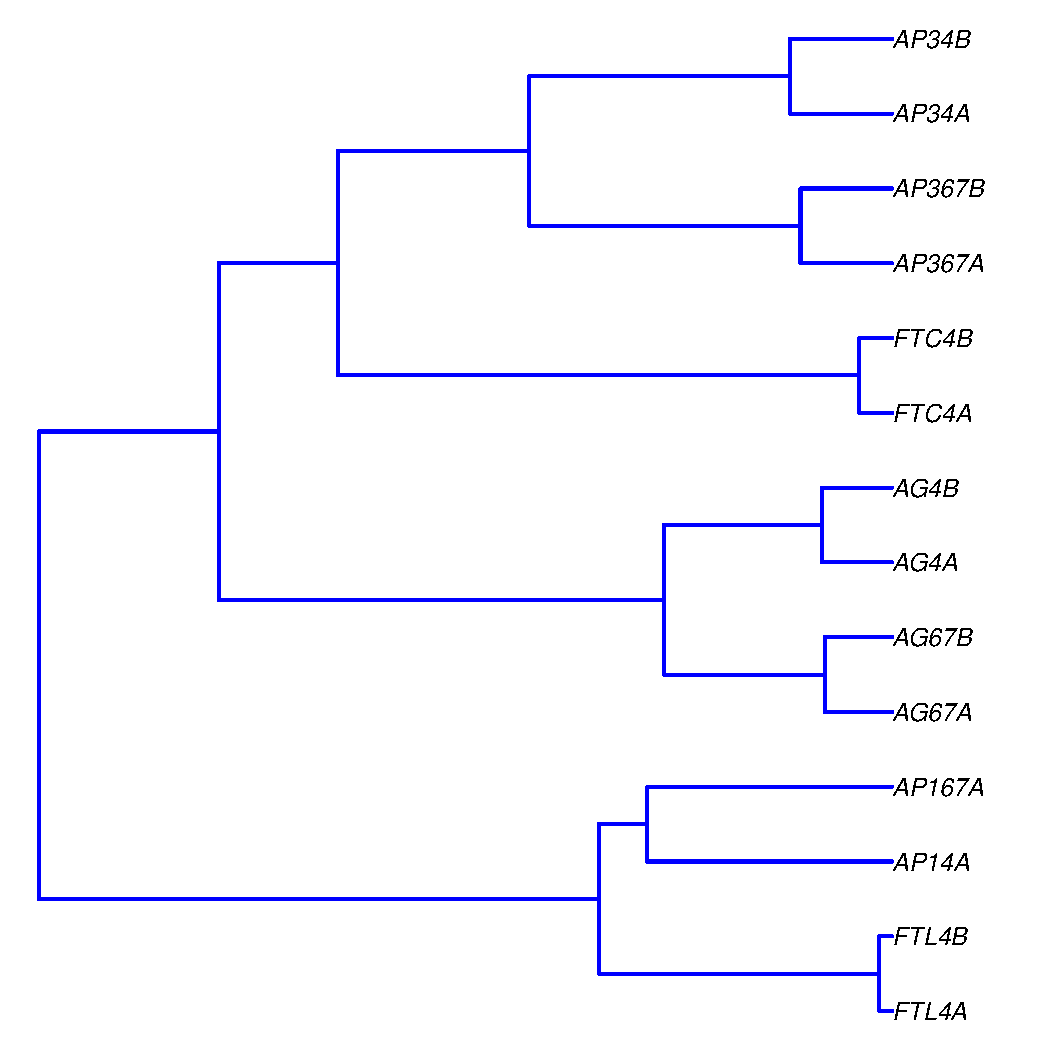
\includegraphics[width=10cm]{sample_tree.pdf}
   \caption{Correlation dendrogram of samples.}
   \label{fig:sample_tree}
\end{figure}

\section{Analysis of differentially expressed genes with \Rpackage{edgeR}}
The analysis of differentially expressed genes (DEGs) is performed with the glm method from the \Rpackage{edgeR} package \citep{Robinson2010-uk}. The sample comparisons used by this analysis are defined in the header lines of the \href{run:targets.txt}{\Robject{targets}} file starting with \texttt{<CMP>}.
\begin{Schunk}
\begin{Sinput}
> library(edgeR)
> countDF <- read.delim("countDFeByg.xls", row.names=1, check.names=FALSE) 
> targets <- read.delim("targets.txt", comment="#")
> cmp <- readComp(file="targets.txt", format="matrix", delim="-")
> edgeDF <- run_edgeR(countDF=countDF, targets=targets, cmp=cmp[[1]], independent=FALSE, mdsplot="")
\end{Sinput}
\end{Schunk}

Add functional descriptions
\begin{Schunk}
\begin{Sinput}
> desc <- read.delim("data/desc.xls") 
> desc <- desc[!duplicated(desc[,1]),]
> descv <- as.character(desc[,2]); names(descv) <- as.character(desc[,1])
> edgeDF <- data.frame(edgeDF, Desc=descv[rownames(edgeDF)], check.names=FALSE)
> write.table(edgeDF, "./results/edgeRglm_allcomp.xls", quote=FALSE, sep="\t", col.names = NA)
\end{Sinput}
\end{Schunk}

Filter and plot DEG results for up and down regulated genes
\begin{Schunk}
\begin{Sinput}
> edgeDF <- read.delim("results/edgeRglm_allcomp.xls", row.names=1, check.names=FALSE) 
> pdf("results/DEGcounts.pdf")
> DEG_list <- filterDEGs(degDF=edgeDF, filter=c(Fold=2, FDR=1))
> dev.off()
> write.table(DEG_list$Summary, "./results/DEGcounts.xls", quote=FALSE, sep="\t", row.names=FALSE)
\end{Sinput}
\end{Schunk}
\begin{figure}[H]
  \centering
   \includegraphics[width=10cm]{DEGcounts.pdf}
   \caption{Up and down regulated DEGs with FDR of 1\%.}
   \label{fig:DEGcounts}
\end{figure}

The function \Rfunction{overLapper} can compute Venn intersects for large numbers of sample sets (up to 20 or more) and \Rfunction{vennPlot} can plot 2-5 way Venn diagrams. A useful feature is the possiblity to combine the counts from several Venn comparisons with the same number of sample sets in a single Venn diagram (here for 4 up and down DEG sets).
\begin{Schunk}
\begin{Sinput}
> vennsetup <- overLapper(DEG_list$Up[6:9], type="vennsets")
> vennsetdown <- overLapper(DEG_list$Down[6:9], type="vennsets")
> pdf("results/vennplot.pdf")
> vennPlot(list(vennsetup, vennsetdown), mymain="", mysub="", colmode=2, ccol=c("blue", "red"))
> dev.off()
\end{Sinput}
\end{Schunk}
\begin{figure}[H]
  \centering
   \includegraphics[width=14cm]{vennplot.pdf}
   \caption{Venn Diagram for 4 Up and Down DEG Sets.}
   \label{fig:vennplot}
\end{figure}

\subsection{GO term enrichment analysis of DEGs}
\subsubsection{Obtain gene-to-GO mappings}
The following shows how to obtain gene-to-GO mappings from \Rpackage{biomaRt} (here for \textit{A. thaliana}) and how to organize them for the downstream GO term enrichment analysis. Alternatively, the gene-to-GO mappings can be obtained for many organisms from Bioconductor's  \Robject{*.db} genome annotation packages or GO annotation files provided by various genome databases. For each annotation this relatively slow preprocessing step needs to be performed only once. Subsequently, the preprocessed data can be loaded with the \Rfunction{load} function as shown in the next subsection. 
\begin{Schunk}
\begin{Sinput}
> library("biomaRt")
> listMarts() # To choose BioMart database
> m <- useMart("ENSEMBL_MART_PLANT"); listDatasets(m) 
> m <- useMart("ENSEMBL_MART_PLANT", dataset="athaliana_eg_gene")
> listAttributes(m) # Choose data types you want to download
> go <- getBM(attributes=c("go_accession", "tair_locus", "go_namespace_1003"), mart=m)
> go <- go[go[,3]!="",]; go[,3] <- as.character(go[,3])
> go[go[,3]=="molecular_function", 3] <- "F"; go[go[,3]=="biological_process", 3] <- "P"; go[go[,3]=="cellular_component", 3] <- "C"
> go[1:4,]
> dir.create("./data/GO")
> write.table(go, "data/GO/GOannotationsBiomart_mod.txt", quote=FALSE, row.names=FALSE, col.names=FALSE, sep="\t")
> catdb <- makeCATdb(myfile="data/GO/GOannotationsBiomart_mod.txt", lib=NULL, org="", colno=c(1,2,3), idconv=NULL)
> save(catdb, file="data/GO/catdb.RData") 
\end{Sinput}
\end{Schunk}

\subsubsection{Batch GO term enrichment analysis}
Apply the enrichment analysis to the DEG sets obtained the above differential expression analysis. Note, in the following example the \Rfunarg{FDR} filter is set here to an unreasonably high value, simply because of the small size of the toy data set used in this vignette. Batch enrichment analysis of many gene sets is performed with the \Rfunction{GOCluster\_Report} function. When \Rfunarg{method="all"}, it returns all GO terms passing the p-value cutoff specified under the \Rfunarg{cutoff} arguments. When \Rfunarg{method="slim"}, it returns only the GO terms specified under the \Rfunarg{myslimv} argument. The given example shows how a GO slim vector for a specific organism can be obtained from BioMart.  
\begin{Schunk}
\begin{Sinput}
> load("data/GO/catdb.RData")
> DEG_list <- filterDEGs(degDF=edgeDF, filter=c(Fold=2, FDR=50), plot=FALSE)
> up_down <- DEG_list$UporDown; names(up_down) <- paste(names(up_down), "_up_down", sep="")
> up <- DEG_list$Up; names(up) <- paste(names(up), "_up", sep="")
> down <- DEG_list$Down; names(down) <- paste(names(down), "_down", sep="")
> DEGlist <- c(up_down, up, down)
> DEGlist <- DEGlist[sapply(DEGlist, length) > 0]
> BatchResult <- GOCluster_Report(catdb=catdb, setlist=DEGlist, method="all", id_type="gene", CLSZ=2, cutoff=0.9, gocats=c("MF", "BP", "CC"), recordSpecGO=NULL)
> library("biomaRt"); m <- useMart("ENSEMBL_MART_PLANT", dataset="athaliana_eg_gene")
> goslimvec <- as.character(getBM(attributes=c("goslim_goa_accession"), mart=m)[,1])
> BatchResultslim <- GOCluster_Report(catdb=catdb, setlist=DEGlist, method="slim", id_type="gene", myslimv=goslimvec, CLSZ=10, cutoff=0.01, gocats=c("MF", "BP", "CC"), recordSpecGO=NULL)
\end{Sinput}
\end{Schunk}

\subsubsection{Plot batch GO term results}
The \Robject{data.frame} generated by \Rfunction{GOCluster\_Report} can be plotted with the \Rfunction{goBarplot} function. Because of the variable size of the sample sets, it may not always be desirable to show the results from different DEG sets in the same bar plot. Plotting single sample sets is achieved by subsetting the input data frame as shown in the first line of the following example. 
\begin{Schunk}
\begin{Sinput}
> gos <- BatchResultslim[grep("M6-V6_up_down", BatchResultslim$CLID), ]
> gos <- BatchResultslim
> pdf("GOslimbarplotMF.pdf", height=8, width=10); goBarplot(gos, gocat="MF"); dev.off()
> goBarplot(gos, gocat="BP")
> goBarplot(gos, gocat="CC")
\end{Sinput}
\end{Schunk}

\begin{figure}[H]
  \centering
   \includegraphics[width=20cm]{GOslimbarplotMF.pdf}
   \caption{GO Slim Barplot for MF Ontology.}
   \label{fig:GOMF}
\end{figure}

\section{Clustering and heat maps}
The following example performs hierarchical clustering on the RPKM normalized expression matrix subsetted by the DEGs identified in the 
above differential expression analysis. It uses a Pearson correlation-based distance measure and complete linkage for cluster joining.
\begin{Schunk}
\begin{Sinput}
> library(pheatmap)
> geneids <- unique(as.character(unlist(DEG_list[[1]])))
> y <- rpkmDFeByg[geneids, ]
> pdf("heatmap1.pdf")
> pheatmap(y, scale="row", clustering_distance_rows="correlation", clustering_distance_cols="correlation")
> dev.off()
\end{Sinput}
\end{Schunk}

\begin{figure}[H]
  \centering
   \includegraphics[width=12cm]{heatmap1.pdf}
   \caption{Heat map with hierarchical clustering dendrograms of DEGs.}
   \label{fig:heatmap}
\end{figure}

\section{Version Information}
\begin{Schunk}
\begin{Sinput}
> toLatex(sessionInfo())
\end{Sinput}
\begin{itemize}\raggedright
  \item R version 3.1.2 (2014-10-31), \verb|x86_64-pc-linux-gnu|
  \item Locale: \verb|LC_CTYPE=en_US.UTF-8|, \verb|LC_NUMERIC=C|, \verb|LC_TIME=en_US.UTF-8|, \verb|LC_COLLATE=en_US.UTF-8|, \verb|LC_MONETARY=en_US.UTF-8|, \verb|LC_MESSAGES=en_US.UTF-8|, \verb|LC_PAPER=en_US.UTF-8|, \verb|LC_NAME=C|, \verb|LC_ADDRESS=C|, \verb|LC_TELEPHONE=C|, \verb|LC_MEASUREMENT=en_US.UTF-8|, \verb|LC_IDENTIFICATION=C|
  \item Base packages: base, datasets, graphics, grDevices, methods, parallel,
    stats, stats4, utils
  \item Other packages: AnnotationDbi~1.28.2, Biobase~2.26.0, BiocGenerics~0.12.1,
    BiocParallel~1.0.3, Biostrings~2.34.1, DBI~0.3.1, GenomeInfoDb~1.2.5,
    GenomicAlignments~1.2.2, GenomicRanges~1.18.4, IRanges~2.0.1, Rsamtools~1.18.3,
    RSQLite~1.0.0, S4Vectors~0.4.0, ShortRead~1.24.0, systemPipeR~1.0.12,
    XVector~0.6.0
  \item Loaded via a namespace (and not attached): annotate~1.44.0,
    AnnotationForge~1.8.2, base64enc~0.1-2, BatchJobs~1.6, BBmisc~1.9,
    BiocStyle~1.4.1, bitops~1.0-6, brew~1.0-6, Category~2.32.0, checkmate~1.5.3,
    codetools~0.2-11, colorspace~1.2-6, digest~0.6.8, edgeR~3.8.6, fail~1.2,
    foreach~1.4.2, genefilter~1.48.1, ggplot2~1.0.1, GO.db~3.0.0, GOstats~2.32.0,
    graph~1.44.1, grid~3.1.2, GSEABase~1.28.0, gtable~0.1.2, hwriter~1.3.2,
    iterators~1.0.7, lattice~0.20-31, latticeExtra~0.6-26, limma~3.22.7,
    magrittr~1.5, MASS~7.3-40, Matrix~1.2-0, munsell~0.4.2, pheatmap~1.0.2,
    plyr~1.8.2, proto~0.3-10, RBGL~1.42.0, RColorBrewer~1.1-2, Rcpp~0.11.6,
    reshape2~1.4.1, rjson~0.2.15, scales~0.2.4, sendmailR~1.2-1, splines~3.1.2,
    stringi~0.4-1, stringr~1.0.0, survival~2.38-1, tools~3.1.2, XML~3.98-1.1,
    xtable~1.7-4, zlibbioc~1.12.0
\end{itemize}\end{Schunk}

\section{Funding}
This project was supported by funds from the National Institutes of Health (NIH).

\bibliography{bibtex}

\end{document}
